\documentclass{beamer}

\usepackage{amsmath}
\usepackage{graphicx}
\usepackage[export]{adjustbox}

\usepackage{xeCJK}  % 导入中文包
% \setCJKmainfont{SimHei}  % 黑体
\setCJKmainfont{Microsoft YaHei}  % 微软雅黑
% \defaultCJKfontfeatures{Scale=0.9}

% 设置Beamer主题
\usetheme{Madrid} %主题
% \usecolortheme{sustech}  % 主题颜色

\usefonttheme[onlymath]{serif}  % 公式字体
% \useoutertheme{noslidenum}

\setbeamertemplate{footline}
{
    \leavevmode
    \hbox{
        \begin{beamercolorbox}[wd=.2\paperwidth,ht=2.5ex,dp=1.5ex,center]{author in head/foot}
            \ifnum \the\value{page}>1 \usebeamerfont{author in head/foot}\insertshortauthor\fi
        \end{beamercolorbox}  % 作者
        \begin{beamercolorbox}[wd=0.6\paperwidth,ht=2.5ex,dp=1.5ex,center]{section in head/foot}
            \usebeamerfont{section in head/foot}\insertsection
        \end{beamercolorbox}  % 章节标题
        \begin{beamercolorbox}[wd=0.2\paperwidth,ht=2.5ex,dp=1.5ex,center]{author in head/foot}
            \ifnum \the\value{page}>1 \insertframenumber{} / \inserttotalframenumber\fi
        \end{beamercolorbox}  % 页码
    }
    \vskip0pt
}

% Information to be included in the title page:
\title{Chapter 4 \\ Lipschitz concentration and transportation inequalities}
\author{童璟}
\date{2023.02.24}

\begin{document}

\frame{\titlepage}

\section{本章内容}
% ----------------------------------------

\begin{frame}{本章内容}
\tableofcontents
\end{frame}

\section{4.1 Concentration in metric spaces}
% ----------------------------------------

\begin{frame}
\begin{center}
\Large Section 4.1 \\ Concentration in metric spaces \\ 度量空间里的集中
\end{center}
\end{frame}

\begin{frame}
\frametitle{4.1节主要内容}
\begin{itemize}
    \item 度量空间和Lipschitz函数
    \item 2个例子:Gaussian集中和McDiarmid不等式
    \item Bobkov-G{\" o}tze定理
    \item 例子:Pinsker不等式
\end{itemize}
\end{frame}

\begin{frame}{度量空间和Lipschitz函数}

\textbf{度量空间(metric space)}:二元组 $(\mathbb{X}, d)$
\begin{itemize}
    \item $\mathbb{X}$ 是集合,是下面函数 $f$ 的定义域
    \item $d: \mathbb{X}\times \mathbb{X} \to \mathbb{R}$ 是距离
\end{itemize}

\quad

\textbf{$L$-Lipschitz函数} $f: \mathbb{X} \to \mathbb{R}$ 满足
$$
\forall x, y \in\mathbb{X}, |f(x) - f(y)| \le L d(x, y)
$$

\textbf{$1$-Lipschitz} 的函数的集合记作 $\text{Lip}(\mathbb{X})$

\end{frame}

\begin{frame}{例子:Gaussian集中(concentration)}

\textbf{定理3.25(Gaussian集中)} $X_1, \cdots, X_n$ 独立同分布 $N(0, 1)$,则对于任意函数 $f$,随机变量 $f(X_1, \cdots, X_n)$ 是 $\|\|\nabla f\|^2\|_{\infty}$-亚高斯($\sigma^2$ 用梯度表示)

\quad

\textbf{重新表述:} $X_1, \cdots, X_n$ 独立同分布 $N(0, 1)$,则只要 $f\in{\rm Lip}(\mathbb{R}^{n}, \|\cdot\|)$,那么$f(X_1, \cdots, X_n)$ 是 $1$-亚高斯($\sigma^2$ 用Lipschitz性质表示)

\quad

\textbf{引理4.3} 设 $f: \mathbb{R}^n \to \mathbb{R}$ 一阶导数连续,则欧氏距离意义下的 $L$-Lipschitz 等价于 $\|\|\nabla f\|^2\|_{\infty} \le L^2$

\end{frame}

\begin{frame}{例子:McDiarmid不等式}

\textbf{“discrete derivative”}
$$
\begin{aligned}
D_i f(x) &:= \sup_{z} f(x_1,\cdots,x_{i-1},z,x_{i+1},\cdots,x_n) \\
&\quad - \inf_{z} f(x_1,\cdots,x_{i-1},z,x_{i+1},\cdots,x_n)
\end{aligned}
$$

\begin{itemize}
    \item 理解为 $f(x)$ 对 $x_i$ 的“离散导数”
    \item 是因 $x_i$ 变化而导致函数 $f(x)$ 值变化量的上确界
\end{itemize}

\textbf{weighted Hamming distance}
$$
d_c(x, y) := \sum_{i=1}^{n} c_i \mathbf{1}_{x_i\neq y_i}
$$

\begin{itemize}
    \item 定义在 $\mathbb{X}_1\times\cdots\times\mathbb{X}_n$ 上,$\mathbb{X}_i$ 可测 $(i=1,\cdots,n)$
    \item 从零开始,第 $i$ 坐标不同则加 $c_i$
\end{itemize}

\end{frame}

\begin{frame}{例子:McDiarmid不等式(续)}

\textbf{定理3.11(McDiarmid不等式)} $X_i\in\mathbb{X}_i$ 相互独立,则对于任意函数 $f$,随机变量 $f(X_1, \cdots, X_n)$ 是 $\frac{1}{4} \sum_{k=1}^{n} \|D_k f\|_{\infty}^2$-亚高斯($\sigma^2$ 用“离散导数”表示)

\quad

\textbf{重新表述:} $X_i\in\mathbb{X}_i$ 相互独立,则只要 $f\in{\rm Lip}(\mathbb{X}_1\times\cdots\times\mathbb{X}_n, d_c)$,那么$f(X_1, \cdots, X_n)$ 是 $\frac{1}{4}\|c\|^2$-亚高斯($\sigma^2$ 用Lipschitz性质表示)

\quad

\textbf{引理4.5} 设 $f: \mathbb{X}_1\times\cdots\times\mathbb{X}_n \to \mathbb{R}$,则 $d_c$ 距离意义下 $1$-Lipschitz 等价于 $\forall i\ ||D_i f||_{\infty} \le c_i$

\end{frame}

\begin{frame}{Bobkov-G{\"o}tze定理}

定义两个概率测度 $\mu, \nu$ 之间的两种“距离”

\begin{center}
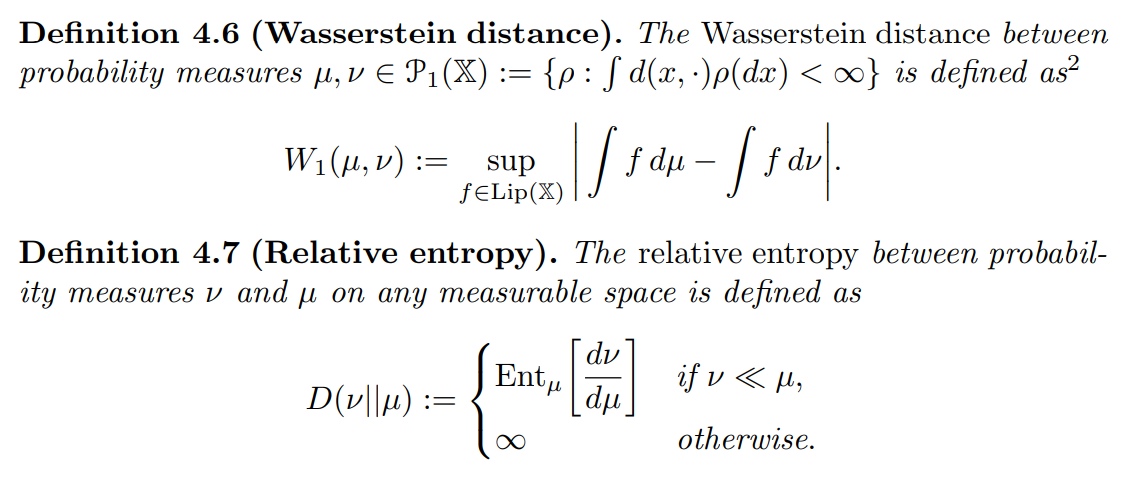
\includegraphics[width=1.0\textwidth, frame]{figures/4-6-def-4-7-def.png}
\end{center}

\end{frame}

\begin{frame}{Bobkov-G{\"o}tze定理(续)}

问题:在度量空间 $(\mathbb{X}, d)$ 中,怎样的概率测度 $\mu$ 能够使任意函数 $f\in{\rm Lip}(\mathbb{X})$,随机变量 $f(X)$ 都是亚高斯?

\begin{center}
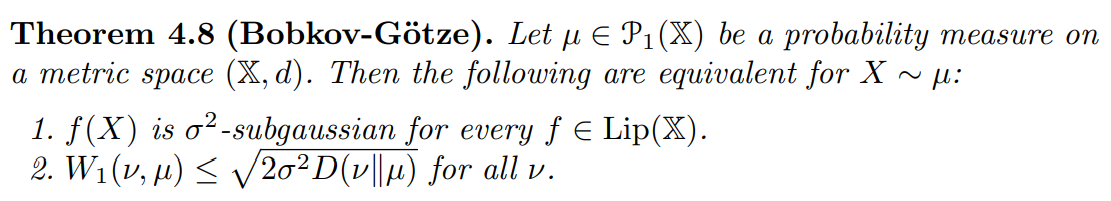
\includegraphics[width=1.0\textwidth, frame]{figures/4-8-thm.png}
\end{center}

证明用到

\begin{center}
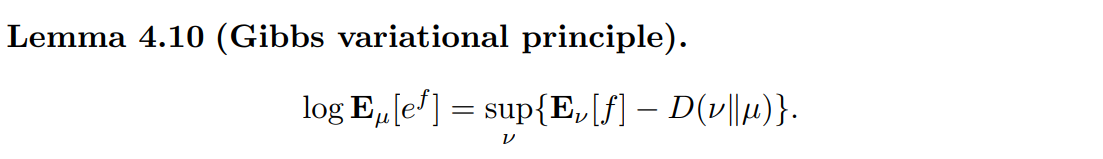
\includegraphics[width=1.0\textwidth, frame]{figures/4-10-lemma.png}
\end{center}

\end{frame}

\begin{frame}{例子:Pinsker不等式}

\textbf{trivial metric} $d(x, y) := \mathbf{1}_{x\neq y}$ 意义下的Lipschitz条件等价于 $|\sup f - \inf f| \le 1$

\textbf{总变差(total variation distance)}

$$
\|\mu-\nu\|_{\rm TV} := \sup_{0\le f\le 1} \left|\int fd\mu - \int fd\nu\right| = W_1(\mu, \nu)
$$

\textbf{Pinsker不等式}

$$
\|\mu-\nu\|_{\rm TV} \le \sqrt{\cfrac{1}{2}D(\nu\|\mu)}
$$

\textbf{引理3.6 (Hoeffding引理)} 有界 $f(X)$ 是 $\frac{1}{4}(\sup f - \inf f)$-亚高斯
    
\end{frame}

\section{4.2 Transportation inequalities and tensorization}
% ----------------------------------------

\begin{frame}
\begin{center}
\Large Section 4.2 \\ Transportation inequalities and tensorization \\ 运输不等式和张量化
\end{center}
\end{frame}

\begin{frame}{4.2节主要内容}

\begin{itemize}
    \item 对偶(duality)和运输(transportation)
    \begin{itemize}
        \item Monge-Kantorovich对偶
        \item 例子:总变差(total variation)
        \item 运输不等式(transportation inequality)
    \end{itemize}
    
    \item 张量化(tensorization)
    \begin{itemize}
        \item Marton定理
        \item 推论
    \end{itemize}
\end{itemize}

\end{frame}

\begin{frame}{Monge-Kantorovich对偶}

\textbf{耦合(Coupling)} $\mathcal{C}(\mu, \nu)$ 是以 $\mu, \nu$ 为边缘分布的联合分布组成的集合

\begin{center}
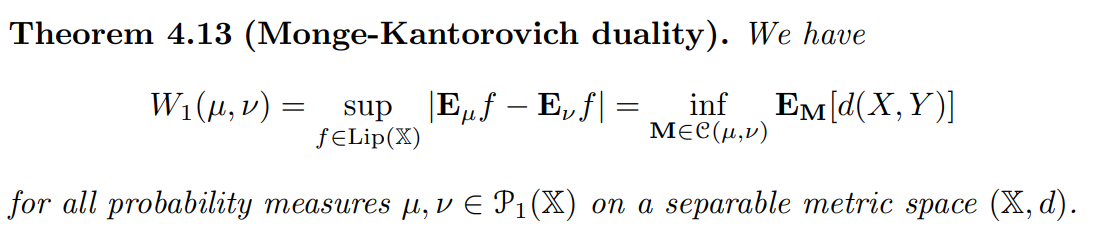
\includegraphics[width=1.0\textwidth, frame]{figures/4-13-thm.png}
\end{center}

optimal transport问题,推土机距离,把两个分布看成两个沙堆,从其中一个形状搬成另一个形状所需的最小成本

\end{frame}

\begin{frame}{例子:总变差(total variation)}

\begin{center}

\includegraphics[width=1.0\textwidth, frame]{figures/4-14-eg.png}
\end{center}

\begin{itemize}
    \item 理解1:搬沙堆最小成本
    \item 理解2:填表格,对角线尽可能大
\end{itemize}

\begin{center}
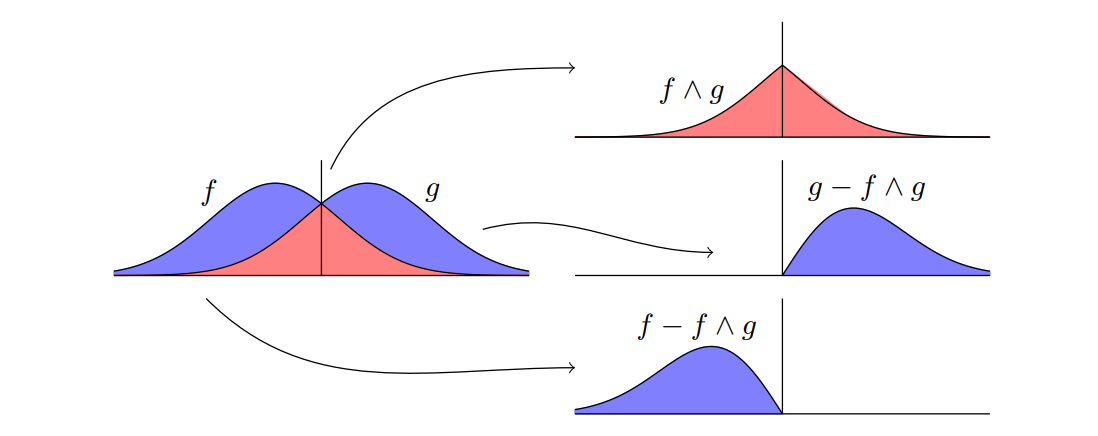
\includegraphics[width=0.8\textwidth, frame]{figures/4-14-fig.png}
\end{center}

\end{frame}

\begin{frame}{运输不等式(transportation inequality)}

把\textbf{Monge-Kantorovich duality}代入\textbf{Bobkov-G{\"o}tze定理},以下1,2等价

1. $X\sim\mu, \forall f\in{\rm Lip}(\mathbb{X})\ f(X)$ 是 $\sigma^2$-亚高斯

2. $\forall \nu\ W_1(\mu, \nu) = \inf_{\mathbf{M} \in \mathcal{C}(\mu,\nu)} \mathbb{E}_{\mathbf{M}} [d(X, Y)] \le \sqrt{2\sigma^{2}D(\nu\|\mu)}$

条件2中的不等式称作\textbf{运输代价不等式(transportation cost inequality)}或\textbf{$T_1$-不等式}

\end{frame}

\begin{frame}{Marton定理}

\begin{center}
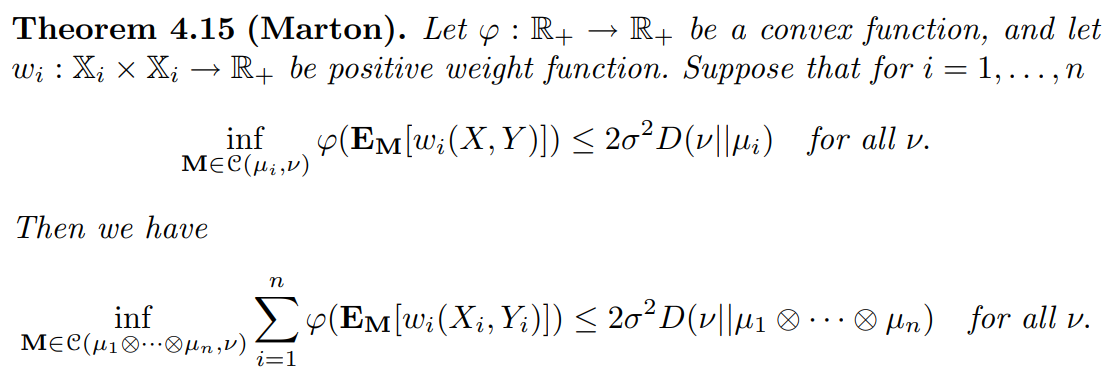
\includegraphics[width=1.0\textwidth, frame]{figures/4-15-thm.png}
\end{center}

\begin{itemize}
    \item 当 $\varphi(x)=x^2, w_i(x, y) = d_i(x, y)$ 时对应运输不等式,左边是Wassersein距离的上界(Cauchy-Schwarz不等式)
    \item 通过 $T_1$ 运输不等式把 $1$ 维亚高斯和 $n$ 维亚高斯联系起来
\end{itemize}

\end{frame}

\begin{frame}{推论}

\textbf{weighted L1 metric} $d_c(x, y) := \sum_{i=1}^{n} c_i d_i(x_i, y_i)$

\begin{center}
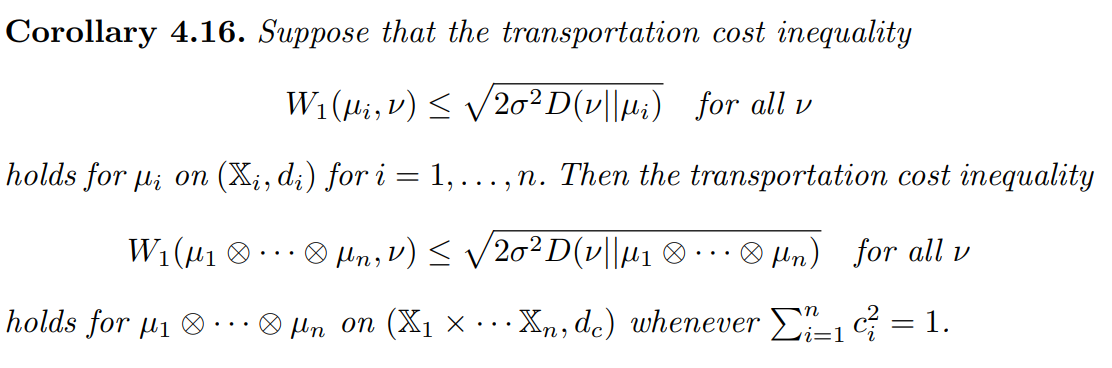
\includegraphics[width=1.0\textwidth, frame]{figures/4-16-corollary.png}
\end{center}

例子:McDiarmid不等式

\end{frame}

\begin{frame}{Marton定理推论和 $T_1$ 不等式图示}
\begin{center}
    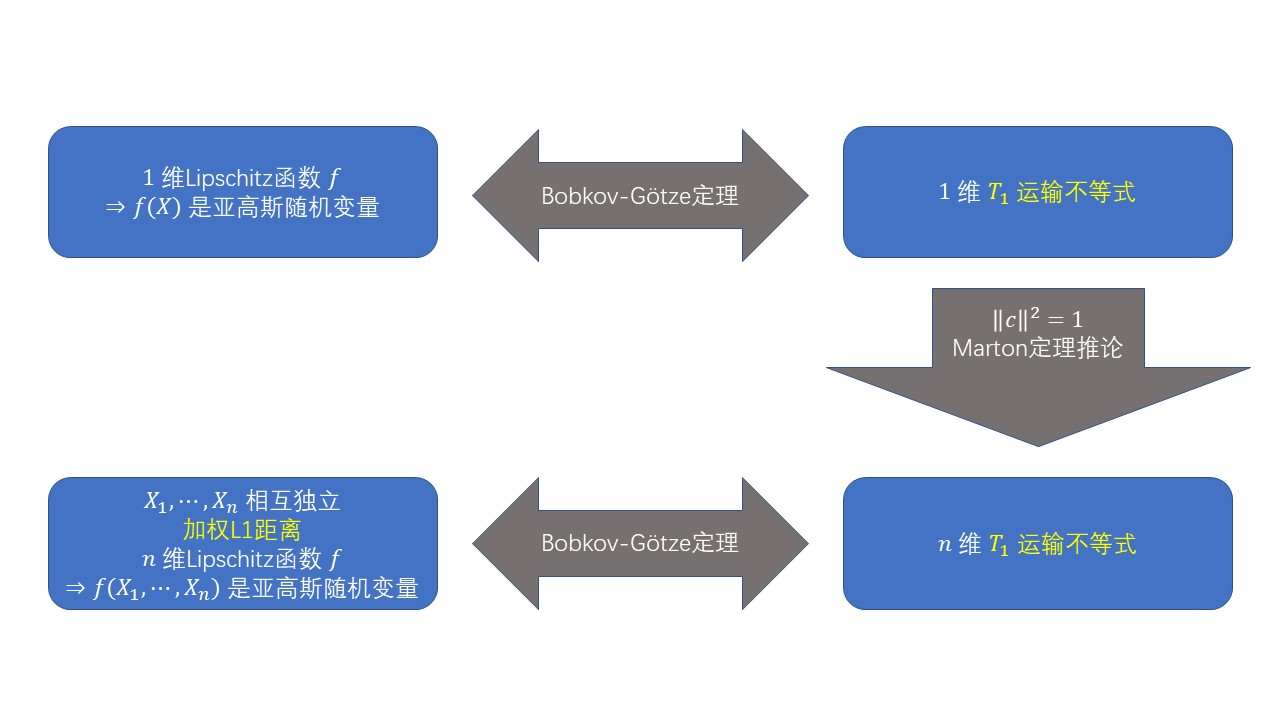
\includegraphics[width=1.0\textwidth]{figures/structure01.JPG}
\end{center}
\end{frame}

\section{4.3 Talagrand's concentration inequality}
% ----------------------------------------

\begin{frame}
\begin{center}
\Large Section 4.3 \\ Talagrand's concentration inequality \\ Talagrand集中不等式
\end{center}
\end{frame}

\begin{frame}{4.3 节主要内容}
\begin{itemize}
    \item 单侧Lipschitz性质
    \item Talagrand定理
    \item 例子:随机矩阵
    \item 推论
\end{itemize}
\end{frame}

\begin{frame}{单侧Lipschitz性质}

回顾1:\textbf{McDiarmid不等式} $X_1, \cdots, X_n$ 相互独立,则

\begin{center}
    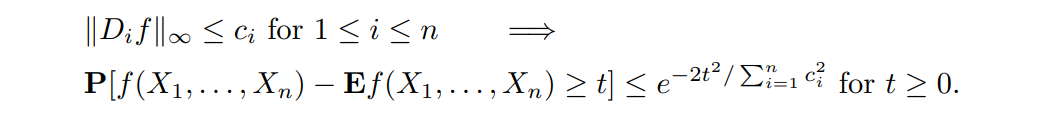
\includegraphics[width=1.0\textwidth, frame]{figures/4-20-001.png}
\end{center}

\begin{itemize}
    \item \textbf{双侧}:$f$ 可以换成 $-f$,符合亚高斯定义,$\sigma^2=\frac{1}{4} \sum_i^n c_i^2$
    \item 上述条件 $\iff$ Lipschitz条件
\end{itemize}

\begin{center}
    
\includegraphics[width=1.0\textwidth, frame]{figures/4-20-003.png}
\end{center}

\end{frame}

\begin{frame}{单侧Lipschitz性质(续)}

回顾2:\textbf{定理3.18} $X_1, \cdots, X_n$ 相互独立,则
\begin{center}
    
\includegraphics[width=1.0\textwidth, frame]{figures/2-4-dminus.png}
    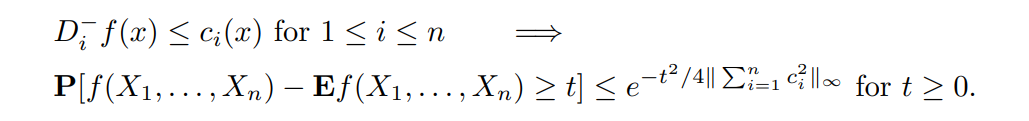
\includegraphics[width=1.0\textwidth, frame]{figures/4-20-002.png}
\end{center}

\begin{itemize}
    \item \textbf{双侧}:若 $D_i^+ f(x)\le c_i(x)$ 且 $D_i^- f(x)\le c_i(x)$,则 $\sigma^2=2\left\|\sum_i^n c_i^2\right\|_{\infty}$
    \item \textbf{单侧}:有时 $D_i^+f, D_i^-f$ 不都有上界,$f$ 不能换成 $-f$,不能得到亚高斯
    \item 上述条件 $\impliedby$ \textbf{“单侧Lipschitz条件”}
\end{itemize}

\begin{center}
    
\includegraphics[width=1.0\textwidth, frame]{figures/4-20-004.png}
\end{center}

\end{frame}

\begin{frame}{Talagrand定理}

由\textbf{单侧}Lipschitz条件得到\textbf{双侧}亚高斯

\begin{center}
    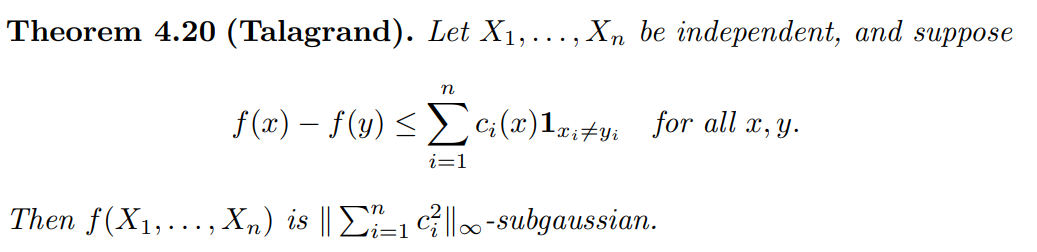
\includegraphics[width=1.0\textwidth, frame]{figures/4-20-thm.png}
\end{center}

在证明本定理的过程中得到了更好的结果

\begin{center}
    
\includegraphics[width=1.0\textwidth, frame]{figures/4-20-better.png}
\end{center}

\end{frame}

\begin{frame}{例子:随机矩阵}

对称 $n\times n$ 矩阵 $M$,独立同分布 $B(1, \frac{1}{2})$,设最大特征值 $\lambda_{\rm max}(M)$,对应特征向量 $v_{\rm max}(M)$

\begin{center}
    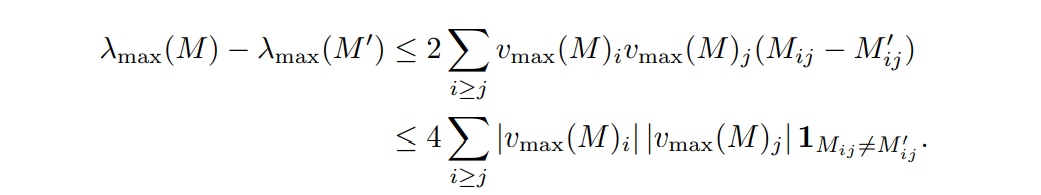
\includegraphics[width=1.0\textwidth, frame]{figures/4-22-eg.png}
\end{center}

函数 $M\mapsto \lambda_{\rm max}(M)$ 满足单侧Lipschitz条件,其中
$$c_{ij}(M) = 4|v_{\rm max}(M)_i||v_{\rm max}(M)_j|$$
由Talagrand定理得 $\sigma^2=16$ 

\end{frame}

\begin{frame}{推论}

\begin{itemize}
    \item Talagrand定理当中的单侧Lipschitz用的是加权Hamming距离
    \item 欧氏距离需要更强的条件:凸函数 $f$,随机变量 $X_1, \cdots X_n$ 有界
\end{itemize}

\begin{center}
    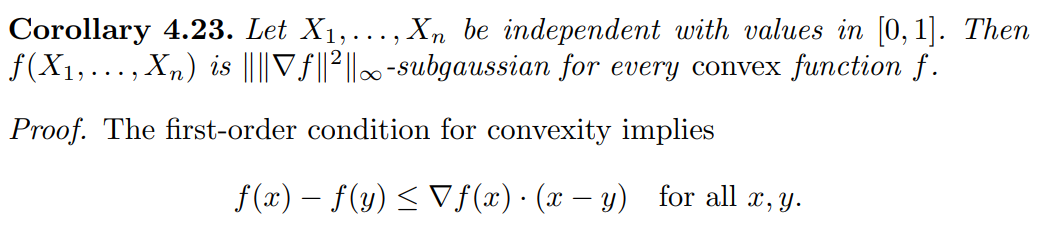
\includegraphics[width=1.0\textwidth, frame]{figures/4-23-corol.png}
\end{center}

\end{frame}

% \begin{frame}{Marton定理}

% \begin{center}
%     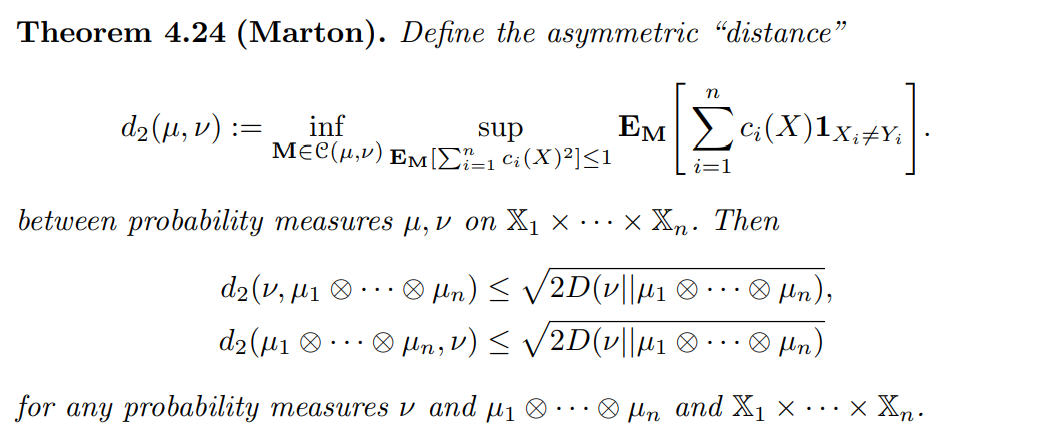
\includegraphics[width=1.0\textwidth, frame]{figures/4-24-thm.png}
% \end{center}

% \end{frame}

\section{4.4 Dimension-free concentration and the \texorpdfstring{$T_2$}{2}-inequality}
% ----------------------------------------

\begin{frame}
\begin{center}
\Large Section 4.4 \\ Dimension-free concentration and the \texorpdfstring{$T_2$}{2}-inequality \\ 维数无关的集中和\texorpdfstring{$T_2$}{2}不等式
\end{center}
\end{frame}

\begin{frame}{4.4 节主要内容}
\begin{itemize}
    \item $T_2$ 不等式
    \item Gozlan定理
\end{itemize}
\end{frame}

\begin{frame}{$T_2$ 不等式}

\begin{center}
    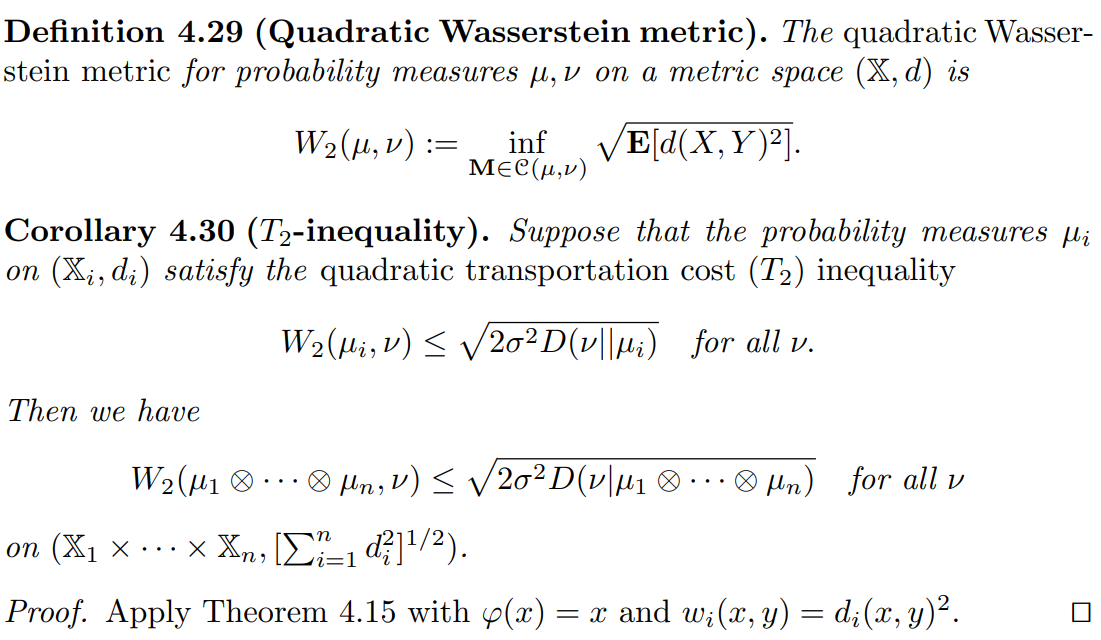
\includegraphics[width=1.0\textwidth, frame]{figures/4-29-def-4-30-corol.png}
\end{center}

\end{frame}

\begin{frame}{对比}

由Jensen不等式得 $W_1(\mu, \nu) \le W_2(\mu, \nu)$

回顾4.2节

\begin{itemize}
    \item 在Marton定理中,令 $\varphi(x)=x^2, w_i(x,y) = d_i(x,y)$
    \item $T_1$ 不等式 $\forall \nu\ W_1(\mu, \nu) \le \sqrt{2\sigma^{2}D(\nu\|\mu)}$ 较弱
    \item 加权L1距离 $d_c(x, y) = \sum_i^n c_i d_i(x_i, y_i)$ 意义下的Lipschitz条件较强
\end{itemize}

本节改进

\begin{itemize}
    \item 在Marton定理中,令 $\varphi(x)=x, w_i(x,y) = d_i(x,y)^2$
    \item $T_2$ 不等式 $\forall \nu\ W_2(\mu, \nu) \le \sqrt{2\sigma^{2}D(\nu\|\mu)}$ 较强
    \item 欧氏距离$d(x, y) = \left[\sum_i^n d_i(x_i, y_i)^2\right]^{1/2}$意义下的Lipschitz条件较弱
\end{itemize}

\end{frame}

\begin{frame}{Marton定理推论 和$T_2$ 不等式图示}
\begin{center}
    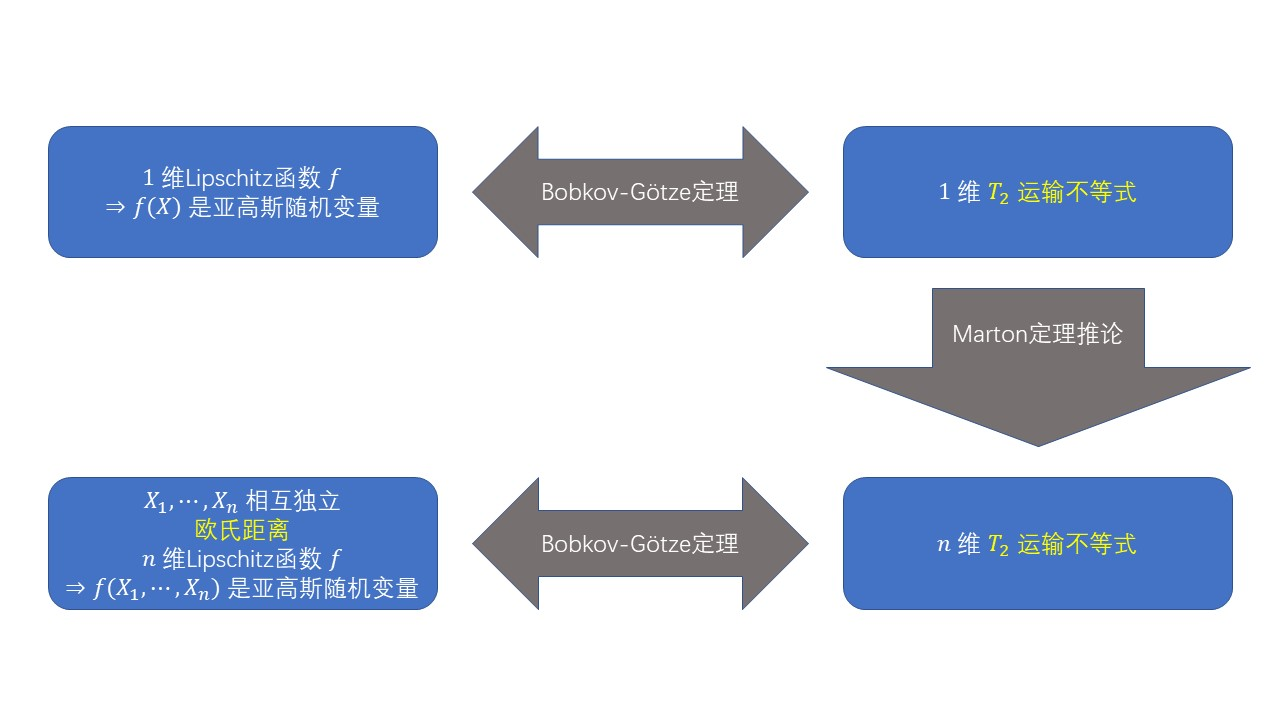
\includegraphics[width=1.0\textwidth]{figures/structure02.JPG}
\end{center}
\end{frame}

\begin{frame}{Gozlan定理}
\begin{center}
    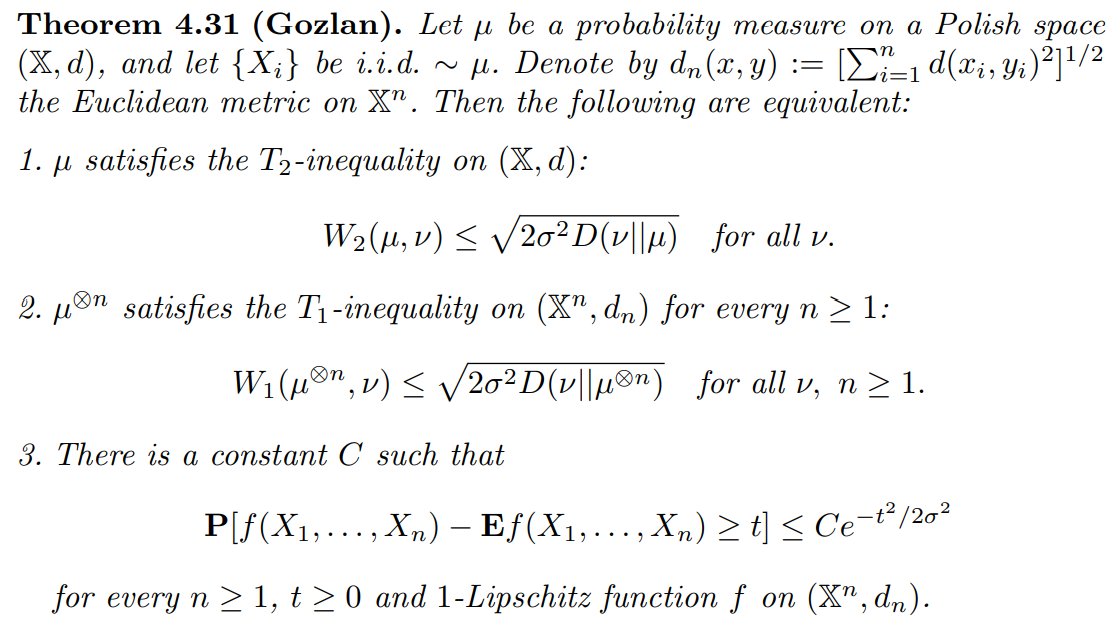
\includegraphics[width=1.0\textwidth, frame]{figures/4-31-thm.png}
\end{center}
\end{frame}

\begin{frame}{Gozlan定理图示}
\begin{center}
    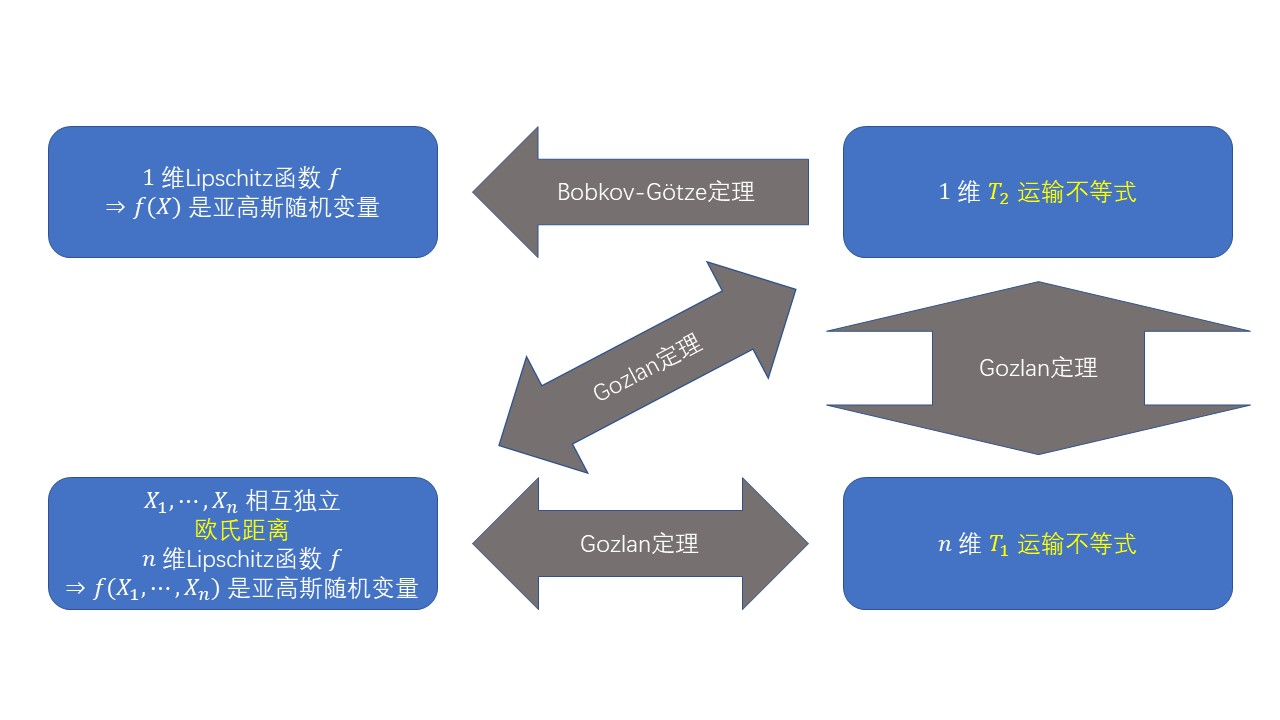
\includegraphics[width=1.0\textwidth]{figures/structure03.JPG}
\end{center}
\end{frame}

\end{document}
